% Gabarit pandoc des corrigés publiés (brut et guidé). Contenu sans marque ni nom de site.
% Compilation : lualatex (latexmk -lualatex).
% Le Markdown reste la source unique : ne pas éditer ce fichier .tex à la main.
\documentclass[11pt,a4paper]{article}

% --- Moteur, polices (Latin Modern) et langue ---------------------------------
\usepackage{iftex}
\ifLuaTeX\else\errmessage{Ce document se compile avec lualatex}\fi
\usepackage{amsmath,amssymb,mathtools}
\usepackage{fontspec}
% mathrm=sym : \mathrm prend ses glyphes dans la police mathématique (ℓ, μ, Ω), comme KaTeX.
\usepackage[math-style=TeX,bold-style=TeX,mathrm=sym]{unicode-math}
% Repli pour les glyphes absents de Latin Modern (indices et exposants Unicode,
% flèches, filets des schémas en texte, symboles) : DejaVu, puis Latin Modern Math
% (ℓ, lettres mathématiques Unicode des légendes).
\directlua{
  luaotfload.add_fallback("repliTexte", {"DejaVuSerif:mode=harf;", "DejaVuSans:mode=harf;", "file:latinmodern-math.otf:mode=harf;"})
  luaotfload.add_fallback("repliMono", {"DejaVuSansMono:mode=harf;", "DejaVuSans:mode=harf;", "file:latinmodern-math.otf:mode=harf;"})
}
\setmainfont{Latin Modern Roman}[RawFeature={fallback=repliTexte}]
\setsansfont{Latin Modern Sans}[RawFeature={fallback=repliTexte}]
\setmonofont{Latin Modern Mono}[RawFeature={fallback=repliMono}]
\setmathfont{Latin Modern Math}
\usepackage[french]{babel}
\frenchsetup{SmallCapsFigTabCaptions=false}

% --- Mise en page --------------------------------------------------------------
\usepackage[a4paper,margin=2.2cm,headheight=14pt,footskip=1.2cm]{geometry}
\usepackage{microtype}
\setlength{\emergencystretch}{4em}
\tolerance=1500
\setlength{\parindent}{0pt}
\setlength{\parskip}{0.55\baselineskip plus 2pt minus 1pt}
\usepackage{xcolor}
% Gris nommés : babel-french rend « ! » actif dans le document.
\definecolor{gris2}{gray}{0.98}
\definecolor{gris3}{gray}{0.97}
\definecolor{gris5}{gray}{0.95}
\definecolor{gris35}{gray}{0.65}
\definecolor{gris40}{gray}{0.60}
\definecolor{gris45}{gray}{0.55}
\definecolor{gris50}{gray}{0.50}
\definecolor{gris55}{gray}{0.45}
\definecolor{gris60}{gray}{0.40}
\definecolor{gris65}{gray}{0.35}
\definecolor{gris70}{gray}{0.30}
\definecolor{gris80}{gray}{0.20}
\definecolor{gris85}{gray}{0.15}
\usepackage{graphicx}
\usepackage{float}
\usepackage{caption}
\captionsetup{font=small,labelformat=empty,justification=centering}
\usepackage{booktabs,longtable,array,multirow,calc}
\usepackage{siunitx}
\sisetup{locale=FR}
\usepackage[version=4]{mhchem}
\usepackage{listings}
\usepackage{fancyhdr}
\usepackage{lastpage}
\usepackage[most]{tcolorbox}
\usepackage{enumitem}
\setlist{nosep,leftmargin=*,topsep=2pt}
\usepackage[hidelinks,unicode]{hyperref}
\usepackage{bookmark}
\hypersetup{pdftitle={Mines-Ponts MP — Informatique (option) 2026},pdfauthor={Rédigé par IA},pdfcreator={LaTeX},pdfsubject={Corrigé guidé}}
\usepackage{xurl}

% --- Pandoc : listes, tableaux, figures ----------------------------------------
\providecommand{\passthrough}[1]{#1}
\providecommand{\tightlist}{\setlength{\itemsep}{0pt}\setlength{\parskip}{0pt}}

\makeatletter
\def\maxwidth{\ifdim\Gin@nat@width>\linewidth\linewidth\else\Gin@nat@width\fi}
\def\maxheight{\ifdim\Gin@nat@height>0.55\textheight 0.55\textheight\else\Gin@nat@height\fi}
\makeatother
\setkeys{Gin}{width=\maxwidth,height=\maxheight,keepaspectratio}
\setcounter{secnumdepth}{-\maxdimen}
\providecommand{\pandocbounded}[1]{#1}
\usepackage{longtable,booktabs,array}

% --- Code (listings) -----------------------------------------------------------
\lstset{
  basicstyle=\ttfamily\small,
  columns=fullflexible,
  keepspaces=true,
  breaklines=true,
  breakatwhitespace=false,
  postbreak=\mbox{\textcolor{gris50}{$\hookrightarrow$}\space},
  frame=single,
  rulecolor=\color{gris35},
  framesep=4pt,
  xleftmargin=5pt,xrightmargin=5pt,
  backgroundcolor=\color{gris3},
  keywordstyle=\bfseries,
  commentstyle=\color{gris65},
  stringstyle=\color{gris80},
  showstringspaces=false,
  tabsize=4,
  extendedchars=true,
  aboveskip=6pt,belowskip=6pt,
}

% --- Macros des corrigés (KaTeX ↔ LaTeX) ---------------------------------------
% Les corrigés sont écrits pour KaTeX : on définit ici ce que KaTeX connaît et
% que LaTeX n'a pas, sans jamais retoucher le Markdown.
\providecommand{\R}{\mathbb{R}}
\providecommand{\N}{\mathbb{N}}
\providecommand{\Z}{\mathbb{Z}}
\providecommand{\Q}{\mathbb{Q}}
\providecommand{\C}{\mathbb{C}}
\providecommand{\dd}{\mathrm{d}}
\providecommand{\llbracket}{\lBrack}
\providecommand{\rrbracket}{\rBrack}
\providecommand{\lBrace}{\lbrace}
\providecommand{\rBrace}{\rbrace}
\providecommand{\Box}{\square}
\providecommand{\Diamond}{\lozenge}
\providecommand{\varnothing}{\emptyset}
\providecommand{\argmax}{\operatorname*{arg\,max}}
\providecommand{\argmin}{\operatorname*{arg\,min}}
\renewcommand{\leq}{\leqslant}
\renewcommand{\geq}{\geqslant}

% Équation hors texte : réduite à la largeur de la ligne si elle déborde.
\newsavebox{\boiteequation}
\newcommand{\equationajustee}[1]{%
  \sbox{\boiteequation}{$\displaystyle #1$}%
  \ifdim\wd\boiteequation>\linewidth
    \[\resizebox{\linewidth}{!}{\usebox{\boiteequation}}\]%
  \else
    \[#1\]%
  \fi}

% --- Encadrés pédagogiques (sobres, lisibles en noir et blanc) -----------------
\tcbset{
  encadre/.style={
    enhanced,breakable,sharp corners,
    colback=white,colframe=gris55,
    boxrule=0.4pt,leftrule=2.2pt,
    left=6pt,right=6pt,top=3pt,bottom=3pt,
    before skip=6pt,after skip=6pt,
    fonttitle=\bfseries\small,coltitle=black,
    attach title to upper,after title={\quad},
    parbox=false,
  }
}
\newtcolorbox{indication}[1]{encadre,colframe=gris45,colback=gris2,title={Indication~#1}}
\newtcolorbox{methode}{encadre,colframe=gris70,title={Méthode}}
\newtcolorbox{piege}{encadre,colframe=gris85,boxrule=0.8pt,leftrule=2.2pt,title={Piège}}
\newtcolorbox{jury}{encadre,colframe=gris60,colback=gris5,title={Jury}}
\newtcolorbox{encadrenote}{encadre,colframe=gris40}

% --- Titres de section ---------------------------------------------------------
\usepackage{titlesec}
\titleformat{\section}{\Large\bfseries}{}{0pt}{}
\titleformat{\subsection}{\large\bfseries}{}{0pt}{}
\titleformat{\subsubsection}{\normalsize\bfseries}{}{0pt}{}
\titlespacing*{\section}{0pt}{14pt plus 4pt minus 2pt}{6pt}
\titlespacing*{\subsection}{0pt}{10pt plus 3pt minus 2pt}{4pt}
\titlespacing*{\subsubsection}{0pt}{8pt plus 2pt minus 2pt}{2pt}

% --- En-tête et pied de page ---------------------------------------------------
\pagestyle{fancy}
\fancyhf{}
\fancyhead[L]{\small\textsc{Corrigé guidé} · Mines-Ponts MP}
\fancyhead[R]{\small Informatique 2026}
\fancyfoot[L]{\footnotesize Corrigé rédigé par IA, non officiel}
\fancyfoot[R]{\footnotesize \thepage\,/\,\pageref*{LastPage}}
\renewcommand{\headrulewidth}{0.4pt}
\renewcommand{\footrulewidth}{0pt}
\fancypagestyle{plain}{\fancyhf{}\fancyfoot[R]{\footnotesize \thepage\,/\,\pageref*{LastPage}}\fancyfoot[L]{\footnotesize Corrigé rédigé par IA, non officiel}\renewcommand{\headrulewidth}{0pt}}

\begin{document}
\thispagestyle{plain}
\begin{center}
  {\small\scshape Corrigé guidé}\par\smallskip
  {\LARGE\bfseries Mines-Ponts MP — Informatique (option) 2026\par}\medskip
  {\large Mines-Ponts · MP · Informatique · 2026\par}
\end{center}
\vspace{2pt}\hrule\vspace{8pt}

\emph{Corrigé rédigé par IA, non officiel. Signalez toute erreur.}

\hypertarget{pruxe9sentation-du-sujet}{%
\section{Présentation du sujet}\label{pruxe9sentation-du-sujet}}

\textbf{Format.} L'épreuve dure 3 heures, sans calculatrice ni aucun dispositif électronique. Le code s'écrit \textbf{en OCaml exclusivement}. Les fonctions des modules \texttt{List} et \texttt{Array} sont permises sans explication, et l'énoncé recommande de s'en tenir aux plus courantes. Le barème tient compte de la clarté et de la concision des programmes. Une annexe donne les règles de déduction naturelle à utiliser. On peut réutiliser le résultat d'une question antérieure même sans l'avoir établi.

\textbf{Thème.} Le sujet construit une \textbf{procédure de décision pour l'arithmétique de Presburger} (entiers naturels, addition, sans multiplication) par des automates.

L'idée centrale est de coder un \(n\)-uplet d'entiers par un mot sur l'alphabet \(\Sigma_n\) des colonnes de \(n\) bits, une lettre par rang binaire, \textbf{poids faible en tête}. Un ensemble de \(n\)-uplets devient un langage, une formule devient un automate, et la vérité d'une formule close se lit sur l'état initial.

\textbf{Découpage.}

\begin{itemize}
\tightlist
\item
  \textbf{Section 1} (Q1 à Q4) : exponentiation rapide et codage binaire des lettres. Questions de mise en route.
\item
  \textbf{Section 2} (Q5 à Q14) : lecture de deux automates sur \(\Sigma_2\), puis la boîte à outils, c'est-à-dire le test de déterminisme, la déterminisation (formelle puis en OCaml), le complémentaire et le produit. Q12 contient le piège principal du sujet.
\item
  \textbf{Section 3} (Q15 à Q17) : l'addition est reconnaissable (automate à retenue, avec preuve), la multiplication ne l'est pas.
\item
  \textbf{Section 4} (Q18 à Q22) : écrire des formules de Presburger, les ramener à une forme simple, deux petites preuves en déduction naturelle.
\item
  \textbf{Section 5} (Q23 à Q30) : zéros non significatifs (\texttt{sans\_zero}), projection d'une ligne (\texttt{automate\_existe}), puis l'algorithme formule → automate, son déroulé à la main, son code, sa preuve et son application aux formules closes.
\end{itemize}

\textbf{Notions du programme.} Automates finis déterministes et non déterministes, déterminisation par sous-ensembles, stabilité par complémentaire et intersection, langages non reconnaissables, preuves par invariant et par induction structurelle, déduction naturelle, programmation OCaml sur tableaux, listes et enregistrements.

\textbf{Notations de ce corrigé.}

\begin{itemize}
\tightlist
\item
  Une lettre de \(\Sigma_2\) est notée \(\binom ab\), une lettre de \(\Sigma_3\) est notée \(\langle a,b,c\rangle\) (lignes 1, 2, 3).
\item
  \(\mathbf{0}\) est la lettre nulle. La ligne \(i\) de l'énoncé est l'indice \(i-1\) du tableau OCaml.
\item
  \(\widehat{\delta}(q,m)\) est l'ensemble des états atteints depuis \(q\) en lisant \(m\).
\end{itemize}

\textbf{Ce qu'en dit le rapport 2026.} Le rapport ne publie pas de statistiques par question, mais il classe les questions.

\begin{itemize}
\tightlist
\item
  \textbf{Bien traitées en général} : Q6, Q7, Q9, Q11, Q18, Q21 et Q24.
\item
  \textbf{Mal réussies alors qu'elles sont abordées} : Q2 (complexité), Q3, Q4, Q5 (double inclusion), Q8, Q10 (question de cours), Q13 (oubli de la déterminisation), Q14, Q15, Q16, Q17 et Q20. Ce sont elles qui départagent les copies.
\item
  \textbf{Peu traitées ou peu abordées} : Q12, Q17, Q19, Q22, Q23 et toute la fin, de Q25 à Q30.
\end{itemize}

Le reproche qui revient le plus est le manque de formalisme. Le rapport écrit : « On constate dans beaucoup de copies le refus du formalisme (même simple) : cela donne des descriptions longues, confuses et des argumentations qui n'en sont pas. »

\textbf{Difficulté et gestion du temps.} Avec 30 questions en 3 heures, il faut compter 6 minutes par question en moyenne. Le sujet est progressif, et la plupart des résultats peuvent être admis pour avancer.

\begin{itemize}
\tightlist
\item
  \textbf{À ne pas laisser passer} : Q1, Q3, Q4, Q7, Q9, Q11, Q13, Q15, Q18, Q21, Q22, Q24, Q30.
\item
  \textbf{Le cœur du sujet} : Q5, Q10, Q12, Q14, Q16, Q23, Q25, Q26 et Q28.
\item
  \textbf{Les plus exigeantes} : Q17 (non-\allowbreak{}reconnaissabilité), Q19 et Q20 (formules sans constantes, aplatissement des termes), Q27 (déroulé long) et Q29 (preuve de correction).
\end{itemize}

La section 5 a été peu abordée : un candidat qui y arrive avec du temps gagne des points que peu d'autres prennent. Il est conseillé de la lire dès le début, car elle explique à quoi servent \texttt{sans\_zero} et la convention « l'état initial est l'état 0 ».

\hypertarget{partie-1-impluxe9mentation-de-quelques-fonctions-utiles}{%
\section{Partie 1 --- Implémentation de quelques fonctions utiles}\label{partie-1-impluxe9mentation-de-quelques-fonctions-utiles}}

On fixe le codage d'une lettre de \(\Sigma_n\) par un entier et on l'implémente. Les outils sont l'exponentiation rapide et la division euclidienne.

\hypertarget{question-1}{%
\subsection{Question 1}\label{question-1}}

\begin{indication}{1}

Exprimez \(2^n\) à partir de \(2^{\lfloor n/2\rfloor}\), en distinguant la parité de \(n\).

\end{indication}

\begin{indication}{2}

Combien de fois l'appel récursif doit-il être évalué dans un même appel ?

\end{indication}

\hypertarget{solution}{%
\subsubsection{Solution}\label{solution}}

\begin{lstlisting}[language=Caml]
(* pow2 n = 2^n, par exponentiation rapide *)
let rec pow2 n =
  if n = 0 then 1
  else
    let p = pow2 (n / 2) in
    if n mod 2 = 0 then p * p else 2 * p * p
\end{lstlisting}

Correction, par récurrence forte. Le cas \(n=0\) donne \(1=2^0\). Pour \(n\ge1\), l'appel sur \(\lfloor n/2\rfloor<n\) renvoie \(p=2^{\lfloor n/2\rfloor}\).

La fonction renvoie alors \(p^2=2^n\) si \(n\) est pair, et \(2p^2=2^{2\lfloor n/2\rfloor+1}=2^n\) si \(n\) est impair.

\begin{jury}

Rapport 2026 : « L'algorithme de calcul rapide des puissances semble trop souvent ignoré. » L'énoncé demande explicitement une récursion en \(O(\log n)\) : une boucle qui multiplie \(n\) fois par 2 ne répond pas à la question.

\end{jury}

\hypertarget{question-2}{%
\subsection{Question 2}\label{question-2}}

\begin{indication}{1}

Comptez les appels : quelle relation lie \(C(n)\) et \(C(\lfloor n/2\rfloor)\) ?

\end{indication}

\begin{indication}{2}

Encadrez \(n\) entre deux puissances de 2 consécutives, et voyez ce que devient l'encadrement pour \(\lfloor n/2\rfloor\).

\end{indication}

\hypertarget{solution-1}{%
\subsubsection{Solution}\label{solution-1}}

Soit \(C(n)\) le nombre d'appels déclenchés par \texttt{pow2\ n}. Chaque appel fait \(O(1)\) opérations hors récursion, et un seul appel récursif. On a
\equationajustee{\begin{aligned}
C(0)&=1,\\
C(n)&=1+C(\lfloor n/2\rfloor)\quad\text{pour } n\ge1.
\end{aligned}}

Montrons par récurrence forte que \(C(n)=\lfloor\log_2n\rfloor+2\) pour \(n\ge1\). On a \(C(1)=2\).

Pour \(n\ge2\), avec \(2^k\le n<2^{k+1}\) et \(k\ge1\), on a \(2^{k-1}\le\lfloor n/2\rfloor<2^k\). Donc \(C(n)=1+(k-1+2)=k+2\).

\equationajustee{\boxed{\text{\text{coût}}=\Theta(\log n)=O(\log n)}}

\begin{piege}

\texttt{pow2\ (\allowbreak{}n/\allowbreak{}2)\allowbreak{}\ *\ pow2\ (\allowbreak{}n/\allowbreak{}2)\allowbreak{}} recalcule deux fois le même appel. On obtient \(C(n)=2C(n/2)+1\), soit un coût \textbf{linéaire}, même si l'argument est divisé par 2 à chaque fois. Il faut nommer le résultat par un \texttt{let}.

\end{piege}

\begin{jury}

Rapport 2026 : « Nous avons trouvé des complexités annoncées comme logarithmiques alors que le code fourni est clairement de complexité linéaire. » La preuve doit porter sur le code écrit, pas sur l'algorithme qu'on avait en tête : comptez les appels effectivement déclenchés.

\end{jury}

\hypertarget{question-3}{%
\subsection{Question 3}\label{question-3}}

\begin{indication}{1}

La convention \(v(u)=\sum_j2^ju_j\) de l'introduction suggère quel ordre des bits ?

\end{indication}

\begin{indication}{2}

Une injection entre deux ensembles finis de même cardinal est une bijection.

\end{indication}

\hypertarget{solution-2}{%
\subsubsection{Solution}\label{solution-2}}

Pour une lettre \(t=(t_1,\dots,t_n)\), de composantes lues de haut en bas, on pose
\equationajustee{\gamma(t)=\sum_{i=1}^n2^{\,i-1}t_i\in[\![0,2^n-1]\!].}

Elle est injective. Si \(s\ne t\), soit \(j\) le plus grand indice où elles diffèrent, avec \(s_j=1\) et \(t_j=0\). Alors
\equationajustee{\gamma(s)-\gamma(t)\ge2^{j-1}-\sum_{i<j}2^{i-1}=1.}

Les deux ensembles ont \(2^n\) éléments, donc \(\gamma\) est bijective. Sa réciproque \(\beta\) associe à \(x\) la lettre \((b_1,\dots,b_n)\) définie par
\equationajustee{\boxed{b_i=\big\lfloor x/2^{\,i-1}\big\rfloor\bmod2\quad\text{pour } i\in[\![1,n]\!]}}
c'est-à-dire l'écriture binaire de \(x\), poids faible en haut. Par exemple, pour \(n=4\), \(\beta(13)\) a pour composantes \(1,0,1,1\).

\begin{piege}

Une bijection avec le poids fort en haut est encore une bijection, mais elle ne s'accorde pas avec \(v\) et rend les questions suivantes incohérentes. Prenez la convention de l'énoncé.

\end{piege}

\begin{jury}

Rapport 2026 : « Des réponses souvent confuses ou imprécises. Le lien avec l'écriture binaire des entiers est cependant majoritairement fait. » Exhiber une bijection, c'est donner une formule explicite, puis justifier qu'elle est bijective (ici : injective entre ensembles de même cardinal).

\end{jury}

\hypertarget{question-4}{%
\subsection{Question 4}\label{question-4}}

\begin{indication}{1}

Divisez successivement par 2 : le reste donne le bit courant.

\end{indication}

\begin{indication}{2}

L'assertion doit exclure aussi les \(x\) négatifs.

\end{indication}

\hypertarget{solution-3}{%
\subsubsection{Solution}\label{solution-3}}

On procède par divisions euclidiennes successives par 2.

\begin{lstlisting}[language=Caml]
(* decompose x n : la lettre beta(x) ; la case i porte le bit de poids 2^i *)
let decompose x n =
  assert (0 <= x && x < pow2 n);
  let t = Array.make n 0 in
  let y = ref x in
  for i = 0 to n - 1 do
    t.(i) <- !y mod 2;
    y := !y / 2
  done;
  t
\end{lstlisting}

Invariant : avant le tour \(i\), on a \texttt{!y} \(=\lfloor x/2^i\rfloor\), et les cases \(j<i\) portent les bits de poids \(2^j\). Le coût est \(\Theta(n)\).

\begin{piege}

\texttt{assert\ (\allowbreak{}x\ \textless{}\ pow2\ n)\allowbreak{}} seul laisse passer les \(x\) négatifs, pour lesquels \texttt{mod} renvoie un reste négatif en OCaml.

\end{piege}

\begin{jury}

Rapport 2026 : « L'algorithme simple (à base de division euclidienne) est très peu cité. » Inutile de chercher plus compliqué que des divisions successives par 2.

\end{jury}

\hypertarget{partie-2-automates-finis-sur-sigma_n}{%
\section{\texorpdfstring{Partie 2 --- Automates finis sur \(\Sigma_n\)}{Partie 2 --- Automates finis sur \textbackslash Sigma\_n}}\label{partie-2-automates-finis-sur-sigma_n}}

On apprend à lire un automate sur des colonnes de bits, puis on implémente les constructions qui serviront de connecteurs logiques : la déterminisation et le complémentaire pour \(\neg\), le produit pour \(\wedge\).

\hypertarget{question-5}{%
\subsection{Question 5}\label{question-5}}

\begin{indication}{1}

Commencez par décrire les mots acceptés comme une expression régulière. Repérez l'état bloquant.

\end{indication}

\begin{indication}{2}

Traduisez la forme obtenue en valeurs : où se trouve l'unique 1 de la ligne 2, et quel est le premier 1 de la ligne 1 ?

\end{indication}

\begin{indication}{3}

Que signifie « la plus grande puissance de 2 qui divise \(v_1(m)\) » lorsque \(v_1(m)=0\) ?

\end{indication}

\hypertarget{solution-4}{%
\subsubsection{Solution}\label{solution-4}}

\textbf{Lecture de \({\mathcal{A}}_1\).} L'automate est déterministe. L'état \(q_2\) n'a pas de transition sortante et n'est pas final, et \(q_1\) est le seul état final.

\begin{itemize}
\tightlist
\item
  Depuis \(q_0\), seule \(\binom00\) boucle, \(\binom11\) mène en \(q_1\), et les deux autres lettres mènent en \(q_2\).
\item
  Depuis \(q_1\), \(\binom00\) et \(\binom10\) bouclent, et les autres lettres mènent en \(q_2\).
\end{itemize}

Donc
\equationajustee{\mathcal{L}({\mathcal{A}}_1)=\Big\{\tbinom00^k\,\tbinom11\,s\ :\ k\in\mathbb{N},\ s\in\big\{\tbinom00,\tbinom10\big\}^*\Big\}.\qquad(\star)}

\begin{figure}[H]
\centering
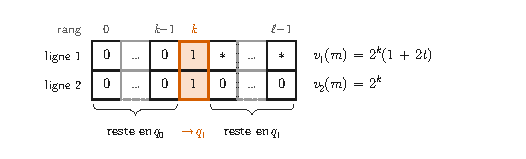
\includegraphics{figures/q5-forme-mots-a1.pdf}
\caption*{Figure 1 --- Forme d'un mot accepté par A₁ : k lettres nulles, la
colonne (1, 1) au rang k, puis une ligne 2 nulle}
\end{figure}

On écrit \(m_j=\binom{u_j}{w_j}\), et on note \(\ell\) la longueur de \(m\).

\textbf{Cas \(v_1(m)=0\).} Toutes les puissances de 2 divisent \(0\), et il n'y en a pas de plus grande : \(m\notin E\). Tout mot de \((\star)\) a un 1 en ligne 1, donc \(m\notin\mathcal{L}({\mathcal{A}}_1)\).

\textbf{Première inclusion, \(\mathcal{L}({\mathcal{A}}_1)\subseteq E\).} Pour \(m\) de la forme \((\star)\), on a \(v_2(m)=2^k\), et \(v_1(m)=2^k(1+2t)\) avec \(t\in\mathbb{N}\).

Donc \(2^k\) divise \(v_1(m)\), \(2^{k+1}\) ne le divise pas, et \(m\in E\).

\textbf{Seconde inclusion, \(E\subseteq\mathcal{L}({\mathcal{A}}_1)\).} Soit \(m\in E\), donc \(v_1(m)\ne0\), et \(2^k\) la plus grande puissance de 2 qui divise \(v_1(m)\). Alors \(v_2(m)=2^k\).

\begin{itemize}
\tightlist
\item
  Comme \(v_2(m)<2^\ell\), on a \(k<\ell\), et l'unicité de l'écriture binaire donne \(w_k=1\) et \(w_j=0\) ailleurs.
\item
  Le premier 1 de la ligne 1, en position \(i_0\), vérifie \(v_1(m)=2^{i_0}(1+2t')\), donc \(i_0=k\).
\end{itemize}

Le mot a la forme \((\star)\), donc il est accepté.

\equationajustee{\boxed{\mathcal{L}({\mathcal{A}}_1)=E}}

\begin{methode}

Pour prouver qu'un automate reconnaît un langage défini arithmétiquement, décrivez d'abord ses mots sous forme régulière. Concluez ensuite par double inclusion, grâce à l'unicité de l'écriture binaire.

\end{methode}

\begin{piege}

Les mots acceptés continuent après la lettre \(\binom11\), avec des lettres dont la ligne 2 est nulle. Il ne faut pas réduire le langage à \(\binom00^k\binom11\).

\end{piege}

\begin{jury}

Rapport 2026 : « Une seule inclusion est souvent citée. La preuve de chaque inclusion est souvent peu convaincante. » Annoncez les deux inclusions par un titre, et démontrez chacune.

\end{jury}

\hypertarget{question-6}{%
\subsection{Question 6}\label{question-6}}

\begin{indication}{1}

Réutilisez l'écriture de \(v_1(m)\) obtenue en Q5.

\end{indication}

\hypertarget{solution-5}{%
\subsubsection{Solution}\label{solution-5}}

Pour \(m\in\mathcal{L}({\mathcal{A}}_1)\), Q5 donne \(v_2(m)=2^k\) et \(v_1(m)=2^k(1+2t)\). Donc
\equationajustee{v_1(m)-v_2(m)=2^{k+1}t=t\cdot2v_2(m),}
d'où
\equationajustee{\boxed{v_1(m)\equiv v_2(m)\ [2\times v_2(m)].}}

\begin{piege}

Le module est \(2v_2(m)\). La congruence modulo \(v_2(m)\) dirait seulement que \(v_2\) divise \(v_1\), ce qui est plus faible.

\end{piege}

\hypertarget{question-7}{%
\subsection{Question 7}\label{question-7}}

\begin{indication}{1}

L'automate est déterministe complet à deux états : chaque état mémorise une information binaire sur le préfixe lu.

\end{indication}

\begin{indication}{2}

En lisant du poids faible au poids fort, quelle lettre décide de la comparaison de deux nombres ?

\end{indication}

\hypertarget{solution-6}{%
\subsubsection{Solution}\label{solution-6}}

\equationajustee{\boxed{\mathcal{L}({\mathcal{A}}_2)=\{m\in\Sigma_2^*:\ v_1(m)>v_2(m)\}}}

L'état \(q_1\) signifie que le préfixe de la ligne 1 vaut strictement plus que celui de la ligne 2.

La lettre \(\binom10\) fait passer en \(q_1\), la lettre \(\binom01\) fait passer en \(q_0\), et une lettre à bits égaux ne change rien. En effet, un bit de poids \(2^j\) l'emporte sur la somme \(2^j-1\) des poids inférieurs.

\begin{piege}

\(q_0\) n'est pas final : le mot vide et les mots à lignes égales sont refusés. La réponse \(v_1\ge v_2\) est donc fausse. Pour vérifier, testez \(\binom10\) (accepté) et \(\binom01\) (refusé).

\end{piege}

\hypertarget{question-8}{%
\subsection{Question 8}\label{question-8}}

\begin{indication}{1}

Pour deux lignes d'un même mot, l'égalité des valeurs équivaut à l'égalité des lignes.

\end{indication}

\begin{indication}{2}

L'automate n'a pas besoin d'être complet. Que suffit-il de mémoriser : lesquelles des deux égalités sont encore possibles ?

\end{indication}

\hypertarget{solution-7}{%
\subsubsection{Solution}\label{solution-7}}

Pour des mots de même longueur, \(v_i(m)=v_j(m)\) équivaut à \(\pi_i(m)=\pi_j(m)\). On reconnaît donc les mots dont toutes les lettres \(\langle a,b,c\rangle\) vérifient \(a=c\), ou dont toutes vérifient \(b=c\).

L'automate est déterministe et incomplet. \(p_0\) est initial, et les trois états sont finaux.

\begin{longtable}[]{@{}
  >{\raggedright\arraybackslash}p{(\columnwidth - 10\tabcolsep) * \real{0.0864}}
  >{\raggedright\arraybackslash}p{(\columnwidth - 10\tabcolsep) * \real{0.2286}}
  >{\raggedright\arraybackslash}p{(\columnwidth - 10\tabcolsep) * \real{0.1883}}
  >{\raggedright\arraybackslash}p{(\columnwidth - 10\tabcolsep) * \real{0.1497}}
  >{\raggedright\arraybackslash}p{(\columnwidth - 10\tabcolsep) * \real{0.1497}}
  >{\raggedright\arraybackslash}p{(\columnwidth - 10\tabcolsep) * \real{0.1673}}@{}}
\toprule\noalign{}
\begin{minipage}[b]{\linewidth}\raggedright
état
\end{minipage} & \begin{minipage}[b]{\linewidth}\raggedright
signification
\end{minipage} & \begin{minipage}[b]{\linewidth}\raggedright
\(a=c \text{ et } b=c\)
\end{minipage} & \begin{minipage}[b]{\linewidth}\raggedright
\(a=c,\ b\ne c\)
\end{minipage} & \begin{minipage}[b]{\linewidth}\raggedright
\(a\ne c,\ b=c\)
\end{minipage} & \begin{minipage}[b]{\linewidth}\raggedright
\(a\ne c,\ b\ne c\)
\end{minipage} \\
\midrule\noalign{}
\endhead
\bottomrule\noalign{}
\endlastfoot
\(p_0\) & les deux égalités tiennent & \(p_0\) & \(p_1\) & \(p_2\) & --- \\
\(p_1\) & seule \(v_1=v_3\) reste possible & \(p_1\) & \(p_1\) & --- & --- \\
\(p_2\) & seule \(v_2=v_3\) reste possible & \(p_2\) & --- & \(p_2\) & --- \\
\end{longtable}

Les lettres de chaque colonne sont :

\begin{itemize}
\tightlist
\item
  \(a=c\) et \(b=c\) : \(\langle0,0,0\rangle\) et \(\langle1,1,1\rangle\) ;
\item
  \(a=c\) et \(b\ne c\) : \(\langle0,1,0\rangle\) et \(\langle1,0,1\rangle\) ;
\item
  \(a\ne c\) et \(b=c\) : \(\langle1,0,0\rangle\) et \(\langle0,1,1\rangle\) ;
\item
  les deux lettres restantes n'ont pas de transition.
\end{itemize}

\begin{figure}[H]
\centering
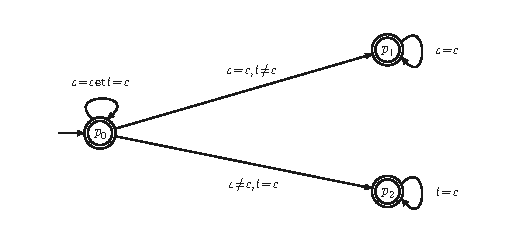
\includegraphics{figures/q8-automate-trois-etats.pdf}
\caption*{Figure 2 --- Automate à trois états pour L, tous finaux : p₀ garde les
deux égalités, p₁ ne suit que v₁ = v₃, p₂ que v₂ = v₃}
\end{figure}

Une variante non déterministe convient aussi.

Depuis \(p_0\), une lettre avec \(a=c\) mène en \(p_1\), une lettre avec \(b=c\) mène en \(p_2\) (éventuellement les deux).

Les états \(p_1\) et \(p_2\) bouclent comme ci-dessus.

\begin{piege}

Si l'on cherche un automate \textbf{complet}, il faut un puits, donc 4 états. La contrainte des 3 états se satisfait en renonçant à la complétude, pas nécessairement au déterminisme. N'oubliez pas que \(\varepsilon\in L\) : l'état initial doit être final.

\end{piege}

\begin{jury}

Rapport 2026 : « Peu de réponse convaincante. Le fonctionnement de l'automate proposé semble rarement bien compris. » Même sans justification demandée, donnez à chaque état sa signification en une phrase : c'est ce qui montre que l'automate est compris.

\end{jury}

\hypertarget{question-9}{%
\subsection{Question 9}\label{question-9}}

\begin{indication}{1}

Énumérez les lettres de \(\Sigma_n\) avec \texttt{decompose}, et testez chaque couple (état, lettre).

\end{indication}

\begin{indication}{2}

Comment tester « liste de longueur exactement 1 » sans parcourir la liste ?

\end{indication}

\hypertarget{solution-8}{%
\subsubsection{Solution}\label{solution-8}}

\begin{lstlisting}[language=Caml]
let est_deterministe_complet a =
  let ok = ref true in
  for x = 0 to pow2 a.n - 1 do
    let lettre = decompose x a.n in   (* chaque lettre construite une fois *)
    for q = 0 to a.k - 1 do
      match a.delta q lettre with
      | [_] -> ()                     (* exactement un successeur *)
      | _ -> ok := false
    done
  done;
  !ok
\end{lstlisting}

Les \(2^n\) valeurs de \(x\) parcourent chaque lettre exactement une fois (Q3). Le filtrage \texttt{{[}\_{]}} reconnaît en \(O(1)\) les listes à un élément.

\textbf{Complexité.} Il y a \(2^n=\lvert\Sigma_n\rvert\) tours. Chacun coûte :

\begin{itemize}
\tightlist
\item
  \(\Theta(n)\) pour construire la lettre ;
\item
  \(\lvert Q\rvert\) appels à \texttt{delta}, en \(O(n)\) chacun (lecture d'une lettre de taille \(n\)), et autant de filtrages en \(O(1)\).
\end{itemize}

Le total vaut
\equationajustee{\boxed{O\big(n\times\lvert Q\rvert\times\lvert\Sigma_n\rvert\big).}}

\begin{piege}

\texttt{List.length\ (\allowbreak{}a.delta\ q\ lettre)\allowbreak{}\ =\allowbreak{}\ 1} parcourt toute la liste, qui peut avoir \(\lvert Q\rvert\) éléments. On peut alors sortir de la borne demandée.

\end{piege}

\begin{jury}

Le rapport 2026 juge la question « bien traitée en général ». Les points se jouent sur la justification demandée : dites ce que coûte un appel à \texttt{delta}, et faites apparaître \(\lvert\Sigma_n\rvert=2^n\) dans le calcul.

\end{jury}

\hypertarget{question-10}{%
\subsection{Question 10}\label{question-10}}

\begin{indication}{1}

Les états de l'automate déterministe sont des ensembles d'états de \(\mathcal{A}\).

\end{indication}

\begin{indication}{2}

Donnez les cinq composantes du tuple. Rencontrer \(F\) et être inclus dans \(F\), ce n'est pas la même chose.

\end{indication}

\hypertarget{solution-9}{%
\subsubsection{Solution}\label{solution-9}}

À \(\mathcal{A}=(\Sigma,Q,q_0,\delta,F)\), on associe \(\mathcal{A}'=\big(\Sigma,\allowbreak \mathcal{P}(Q),\allowbreak \{q_0\},\allowbreak \delta',\allowbreak F'\big)\), où
\equationajustee{\begin{aligned}
\delta'(S,a)&=\Big\{\textstyle\bigcup_{q\in S}\delta(q,a)\Big\}\qquad\text{pour } S\subseteq Q,\ a\in\Sigma,\\
F'&=\{S\subseteq Q:\ S\cap F\ne\emptyset\}.
\end{aligned}}

\(\delta'\) renvoie un singleton, donc \(\mathcal{A}'\) est déterministe complet, et \(\emptyset\) en est le puits.

Par récurrence sur \(\lvert m\rvert\), l'état atteint en lisant \(m\) est \(\widehat{\delta}(q_0,m)\).

Donc \(m\) est accepté par \(\mathcal{A}'\) si et seulement si \(\widehat{\delta}(q_0,m)\cap F\ne\emptyset\), c'est-à-dire si et seulement si \(m\in\mathcal{L}(\mathcal{A})\).

\begin{methode}

Le lemme « l'état atteint dans \(\mathcal{A}'\) est l'ensemble des états atteints dans \(\mathcal{A}\) » se prouve en trois lignes par récurrence sur la longueur. Il resservira pour Q12, Q13 et Q29.

\end{methode}

\begin{jury}

Rapport 2026 : « Question de cours. Le refus du formalisme est ici manifeste. Cela donne des réponses approximatives, très lourdes et souvent incomplètes. » Une construction formelle, c'est le tuple complet, avec l'état initial, la transition et les finaux définis par des formules. Une phrase qui évoque vaguement des ensembles d'états ne suffit pas.

\end{jury}

\hypertarget{question-11}{%
\subsection{Question 11}\label{question-11}}

\begin{indication}{1}

Allouez un tableau neuf, puis marquez les successeurs de chaque état présent.

\end{indication}

\hypertarget{solution-10}{%
\subsubsection{Solution}\label{solution-10}}

\begin{lstlisting}[language=Caml]
let union etats a lettre =
  let t = Array.make a.k 0 in
  for q = 0 to a.k - 1 do
    if etats.(q) = 1 then
      List.iter (fun i -> t.(i) <- 1) (a.delta q lettre)
  done;
  t
\end{lstlisting}

\texttt{t.(i)} vaut 1 si et seulement s'il existe \(q\) marqué dans \texttt{etats} avec \(i\in\delta(q,\texttt{lettre})\). On renvoie bien des entiers 0/1, comme l'impose la signature, et \texttt{etats} n'est pas modifié.

\hypertarget{question-12}{%
\subsection{Question 12}\label{question-12}}

\begin{indication}{1}

Codez une partie de \(Q\) par un entier, par exemple via \texttt{decompose} et sa réciproque.

\end{indication}

\begin{indication}{2}

Relisez la définition du type \texttt{automate} : quel état est toujours initial ? Quel est le code de \(\{q_0\}\) dans votre codage ?

\end{indication}

\begin{indication}{3}

Un renommage bijectif des états ne change pas le langage.

\end{indication}

\hypertarget{solution-11}{%
\subsubsection{Solution}\label{solution-11}}

La partie \(S\) est codée par \(\sum_{q\in S}2^q\).

Mais l'état initial doit être \(0\), alors que \(\{q_0\}\) a pour code \(1\) et que \(0\) code \(\emptyset\).

On compose donc avec la transposition qui échange \(0\) et \(1\).

\begin{lstlisting}[language=Caml]
(* code t : entier dont t est l'ecriture binaire (bit q de poids 2^q) *)
let code t =
  let s = ref 0 in
  for q = Array.length t - 1 downto 0 do
    s := 2 * !s + t.(q)
  done;
  !s

(* transposition 0 <-> 1, involutive *)
let echange x = if x = 0 then 1 else if x = 1 then 0 else x

let determinise a =
  let nb = pow2 a.k in
  let ens x = decompose (echange x) a.k in   (* partie representee par l'etat x *)
  let num t = echange (code t) in            (* etat representant la partie t *)
  let finaux = Array.make nb false in
  for x = 0 to nb - 1 do
    let t = ens x in
    for q = 0 to a.k - 1 do
      if t.(q) = 1 && a.finaux.(q) then finaux.(x) <- true
    done
  done;
  { k = nb; n = a.n; finaux = finaux;
    delta = (fun x lettre -> [ num (union (ens x) a lettre) ]) }
\end{lstlisting}

\texttt{ens} et \texttt{num} sont des bijections réciproques entre \([\![0,2^k-1]\!]\) et les parties de \(Q\). L'automate obtenu est donc celui de Q10, à un renommage près :

\begin{itemize}
\tightlist
\item
  l'état \(0\) représente \(\{q_0\}\) ;
\item
  chaque transition renvoie un singleton ;
\item
  un état est final si et seulement si sa partie rencontre \(F\).
\end{itemize}

Il est déterministe complet et reconnaît \(\mathcal{L}(\mathcal{A})\).

\begin{piege}

Sans la transposition, l'état initial représenterait \(\emptyset\), et l'automate reconnaîtrait le langage vide. Le code compile et l'erreur est silencieuse. Le défaut se propagerait jusqu'à Q30, qui lit justement \texttt{finaux.(0)}.

\end{piege}

\begin{methode}

Pour représenter un automate dont les états sont des objets structurés (parties, couples), choisissez une bijection explicite avec \([\![0,K-1]\!]\). Vérifiez ensuite qu'elle respecte les conventions imposées, ici l'état initial numéroté 0.

\end{methode}

\begin{jury}

Le rapport 2026 note une question « peu traitée ». Ses remarques générales s'appliquent pleinement à ce long code : il recommande « d'utiliser des noms significatifs à l'image de ce que font les concepteurs des sujets », puis : « Un commentaire additionnel permet de mieux évaluer la compréhension du sujet ou de la question par les candidats. » Des fonctions auxiliaires nommées (\texttt{code}, \texttt{echange}, \texttt{ens}, \texttt{num}) rendent la correction lisible.

\end{jury}

\hypertarget{question-13}{%
\subsection{Question 13}\label{question-13}}

\begin{indication}{1}

Échanger finaux et non-finaux ne marche que sous deux hypothèses sur l'automate. Lesquelles ?

\end{indication}

\hypertarget{solution-12}{%
\subsubsection{Solution}\label{solution-12}}

On commence par déterminiser (et compléter), puis on échange finaux et non-finaux.

\begin{lstlisting}[language=Caml]
let complementaire a =
  let d = determinise a in
  { d with finaux = Array.map not d.finaux }
\end{lstlisting}

Dans l'automate déterministe complet \texttt{d}, tout mot a un unique chemin issu de l'état initial. Il est accepté après échange si et seulement s'il était refusé par \texttt{d}, c'est-à-dire si et seulement si \(m\notin\mathcal{L}(\mathcal{A})\).

\begin{piege}

Sur un automate non déterministe, l'échange échoue. Par exemple, sur \(\{a\}\), l'automate \(p_0\xrightarrow{a}p_0\), \(p_0\xrightarrow{a}p_1\), avec \(F=\{p_1\}\), reconnaît \(a^+\). Après échange, il reconnaît \(a^*\). Sur un automate déterministe incomplet, les mots bloqués restent refusés. Il faut donc déterminiser \textbf{et} compléter, ce que fait \texttt{determinise}.

\end{piege}

\begin{jury}

Rapport 2026 : « Beaucoup de candidats oublient de déterminiser l'automate. » La fonction reçoit un automate quelconque : l'appel à \texttt{determinise} n'est pas facultatif.

\end{jury}

\hypertarget{question-14}{%
\subsection{Question 14}\label{question-14}}

\begin{indication}{1}

Faites fonctionner les deux automates en parallèle sur le même mot.

\end{indication}

\begin{indication}{2}

Dans le cas non déterministe, les successeurs d'un couple forment un produit cartésien. Prouvez l'invariant sur \(\widehat{\delta}\) par récurrence sur la longueur.

\end{indication}

\hypertarget{solution-13}{%
\subsubsection{Solution}\label{solution-13}}

Avec \({\mathcal{A}}_1=(\Sigma_n,Q_1,q_1,\delta_1,F_1)\) et \({\mathcal{A}}_2=(\Sigma_n,Q_2,q_2,\delta_2,F_2)\), on pose
\equationajustee{\boxed{\mathcal{P}=\big(\Sigma_n,Q_1\times Q_2,(q_1,q_2),\delta,F_1\times F_2\big)}}
où, pour \((p,q)\in Q_1\times Q_2\) et \(a\in\Sigma_n\),
\equationajustee{\delta((p,q),a)=\delta_1(p,a)\times\delta_2(q,a).}

Les objets ont la bonne nature : \((q_1,q_2)\) est un état, \(F_1\times F_2\) est une partie de \(Q_1\times Q_2\), et \(\delta\) va de \((Q_1\times Q_2)\times\Sigma_n\) dans \(\mathcal{P}(Q_1\times Q_2)\).

Par récurrence sur \(\lvert m\rvert\), on montre que
\equationajustee{\widehat{\delta}((q_1,q_2),m)=\widehat{\delta_1}(q_1,m)\times\widehat{\delta_2}(q_2,m).}

Le cas \(\varepsilon\) est immédiat.

Pour l'hérédité, \((r,s)\) est atteint en lisant \(ma\) si et seulement s'il existe un couple \((p,q)\) atteint en lisant \(m\) tel que \(r\in\delta_1(p,a)\) et \(s\in\delta_2(q,a)\).

Les deux choix sont indépendants.

Donc \(m\) est accepté si et seulement s'il existe \(r\in\widehat{\delta_1}(q_1,m)\cap F_1\) et \(s\in\widehat{\delta_2}(q_2,m)\cap F_2\). Cela signifie \(m\in\mathcal{L}({\mathcal{A}}_1)\cap\mathcal{L}({\mathcal{A}}_2)\).

\begin{piege}

Prendre \((F_1\times Q_2)\cup(Q_1\times F_2)\) donne l'union, pas l'intersection. Pour l'union, cette construction n'est d'ailleurs correcte que si les deux automates sont complets.

\end{piege}

\begin{jury}

Rapport 2026 : « A nouveau, ici, le formalisme est trop superficiel ou bien donne des réponses incohérentes avec la nature des objets manipulés. » Contrôlez les types : \(\delta\) renvoie une \textbf{partie} de \(Q_1\times Q_2\), pas un couple d'ensembles ni un état.

\end{jury}

\hypertarget{partie-3-opuxe9rations-arithmuxe9tiques}{%
\section{Partie 3 --- Opérations arithmétiques}\label{partie-3-opuxe9rations-arithmuxe9tiques}}

On montre que l'addition se calcule avec une mémoire finie (la retenue), alors que la multiplication demande une mémoire non bornée. C'est la raison pour laquelle la méthode s'arrête à l'arithmétique de Presburger.

\hypertarget{question-15}{%
\subsection{Question 15}\label{question-15}}

\begin{indication}{1}

Posez une addition binaire à la main, des poids faibles vers les poids forts. Que faut-il retenir d'une colonne à la suivante ?

\end{indication}

\begin{indication}{2}

Dans quel état faut-il être à la fin pour que l'égalité soit exacte ?

\end{indication}

\hypertarget{solution-14}{%
\subsubsection{Solution}\label{solution-14}}

Les états sont les retenues \(r_0\) (initial, final) et \(r_1\) (non final). La transition est
\equationajustee{\delta_+(r_e,\langle a,b,c\rangle)=\begin{cases}\{r_{e'}\}&\text{si } a+b+e=c+2e',\ e'\in\{0,1\},\\ \emptyset&\text{si } a+b+e\not\equiv c\ [2].\end{cases}}

Chaque état a exactement quatre transitions sortantes, une par lettre de bonne parité :

\begin{longtable}[]{@{}
  >{\raggedright\arraybackslash}p{(\columnwidth - 4\tabcolsep) * \real{0.0713}}
  >{\raggedright\arraybackslash}p{(\columnwidth - 4\tabcolsep) * \real{0.4494}}
  >{\raggedright\arraybackslash}p{(\columnwidth - 4\tabcolsep) * \real{0.4494}}@{}}
\toprule\noalign{}
\begin{minipage}[b]{\linewidth}\raggedright
état
\end{minipage} & \begin{minipage}[b]{\linewidth}\raggedright
vers \(r_0\)
\end{minipage} & \begin{minipage}[b]{\linewidth}\raggedright
vers \(r_1\)
\end{minipage} \\
\midrule\noalign{}
\endhead
\bottomrule\noalign{}
\endlastfoot
\(r_0\) & \(\langle0,\allowbreak 0,\allowbreak 0\rangle,\allowbreak \ \langle1,\allowbreak 0,\allowbreak 1\rangle,\allowbreak \ \langle0,\allowbreak 1,\allowbreak 1\rangle\) & \(\langle1,1,0\rangle\) \\
\(r_1\) & \(\langle0,0,1\rangle\) & \(\langle1,\allowbreak 0,\allowbreak 0\rangle,\allowbreak \ \langle0,\allowbreak 1,\allowbreak 0\rangle,\allowbreak \ \langle1,\allowbreak 1,\allowbreak 1\rangle\) \\
\end{longtable}

Les autres couples (état, lettre) n'ont pas de transition.

\begin{figure}[H]
\centering
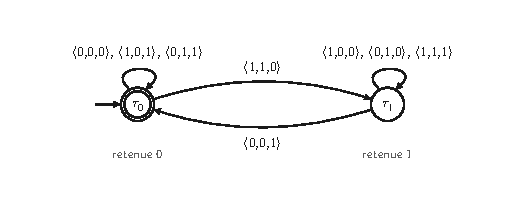
\includegraphics{figures/q15-automate-retenue.pdf}
\caption*{Figure 3 --- Automate de l'addition : l'état est la retenue, seul r₀ est
final}
\end{figure}

\begin{piege}

Rendre \(r_1\) final reviendrait à accepter \(v_1+v_2=v_3+2^{\lvert m\rvert}\), c'est-à-dire un débordement hors du mot. Ajouter un puits pour compléter l'automate coûterait un troisième état, alors que l'énoncé en demande deux.

\end{piege}

\begin{piege}

Ne devinez pas les transitions de \(r_1\) par symétrie avec celles de \(r_0\) : pour chacune des huit lettres, calculez \(a+b+e\) et vérifiez qu'il vaut \(c+2e'\).

\end{piege}

\begin{jury}

Rapport 2026 : « L'idée semble comprise mais les candidats ne vont pas jusqu'à son terme : les premières transitions sont souvent correctes mais les suivantes sont souvent bâclées et fausses. » Un tableau état × lettre, rempli systématiquement, évite les oublis.

\end{jury}

\hypertarget{question-16}{%
\subsection{Question 16}\label{question-16}}

\begin{indication}{1}

Formulez un invariant sur les valeurs des préfixes : que vaut \(A_j+B_j-C_j\) quand on est en \(r_e\) après \(j\) lettres ?

\end{indication}

\begin{indication}{2}

La retenue a pour poids \(2^j\). Pour la réciproque, un encadrement de \(A_j+B_j-C_j\) force la valeur de \(e\).

\end{indication}

\hypertarget{solution-15}{%
\subsubsection{Solution}\label{solution-15}}

Pour \(m_j=\langle a_j,b_j,c_j\rangle\), posons \(A_j=\sum_{l<j}2^la_l\), et de même \(B_j\) et \(C_j\). Ces valeurs sont dans \([\![0,2^j-1]\!]\), donc
\equationajustee{-2^j<A_j+B_j-C_j<2^{j+1}.\qquad({\mathrm{B}}_j)}

\textbf{Invariant} \((I_j)\) : l'ensemble des états atteints après \(j\) lettres est
\equationajustee{S_j=\{r_e:\ A_j+B_j=C_j+e\,2^j\}.}

\begin{itemize}
\tightlist
\item
  \textbf{Initialisation.} \(S_0=\{r_0\}\), et \(0=0+e\) impose \(e=0\).
\item
  \textbf{Hérédité}, avec \(m_j=\langle a,b,c\rangle\). On a \(r_{e'}\in S_{j+1}\) si et seulement s'il existe \(r_e\in S_j\) avec \(a+b+e=c+2e'\).

  \begin{itemize}
  \tightlist
  \item
    Si c'est le cas, on calcule :
    \equationajustee{\begin{aligned}
    A_{j+1}+B_{j+1}&=C_j+2^j(a+b+e)\\
    &=C_j+2^j(c+2e')\\
    &=C_{j+1}+e'2^{j+1}.
    \end{aligned}}
  \item
    Réciproquement, si \(A_{j+1}+B_{j+1}=C_{j+1}+e'2^{j+1}\), on pose \(e=c+2e'-a-b\). Alors \(A_j+B_j-C_j=e2^j\).
  \item
    L'encadrement \(({\mathrm{B}}_j)\) impose \(e\in\{0,1\}\), donc \(r_e\in S_j\).
  \end{itemize}
\end{itemize}

Les blocages sont couverts : si aucune transition n'existe, \(S_{j+1}=\emptyset\), et aucune égalité n'est possible.

Pour \(j=\lvert m\rvert\), \(m\) est accepté si et seulement si \(r_0\in S_{\lvert m\rvert}\), c'est-à-dire si et seulement si \(v_1(m)+v_2(m)=v_3(m)\).

\equationajustee{\boxed{\mathcal{L}({\mathcal{A}}_+)=L_+}}

\begin{methode}

Pour prouver un automate « arithmétique », donnez un sens numérique précis à chaque état sur les préfixes, avec le poids \(2^j\) de ce qui reste à reporter. Démontrez ensuite une \textbf{équivalence} à chaque pas, ce qui donne les deux inclusions d'un coup.

\end{methode}

\begin{jury}

Rapport 2026 : « Peu de preuves convaincantes. » Un exemple d'addition posée ne prouve rien : il faut un invariant énoncé par une formule, puis une récurrence sur la longueur.

\end{jury}

\hypertarget{question-17}{%
\subsection{Question 17}\label{question-17}}

\begin{indication}{1}

La réponse est non. Cherchez des mots de \(L_\times\) qui commencent par beaucoup de lettres nulles.

\end{indication}

\begin{indication}{2}

Que deviennent \(v_1\), \(v_2\) et \(v_3\) si l'on insère \(t\) lettres nulles au début ? Comparez avec ce que devient le produit \(v_1v_2\).

\end{indication}

\begin{indication}{3}

Énoncez précisément le lemme de l'étoile, avec la contrainte sur la longueur du préfixe.

\end{indication}

\hypertarget{solution-16}{%
\subsubsection{Solution}\label{solution-16}}

\textbf{\(L_\times\) n'est pas reconnaissable.}

\textbf{Lemme de l'étoile.} Si un langage \(L\) est reconnu par un automate à \(N\) états, alors tout mot \(m\in L\) de longueur \(\ge N\) s'écrit \(m=xyz\) avec :

\begin{itemize}
\tightlist
\item
  \(\lvert xy\rvert\le N\) ;
\item
  \(y\neq\varepsilon\) ;
\item
  \(xy^kz\in L\) pour tout \(k\in\mathbb{N}\).
\end{itemize}

Il se démontre par le principe des tiroirs sur les \(N+1\) premiers états d'un chemin acceptant.

\textbf{Application.} Supposons \(L_\times\) reconnu par un automate à \(N\) états, et posons \(p=N\). Soit \(m\) le mot de longueur \(2p+1\) défini par
\equationajustee{\begin{aligned}
\pi_1(m)&=0^p\,1\,0^p,\\
\pi_2(m)&=0^p\,1\,0^p,\\
\pi_3(m)&=0^{2p}\,1 .
\end{aligned}}

On a \(v_1=v_2=2^p\) et \(v_3=2^{2p}\), donc \(m\in L_\times\).

Le lemme donne \(m=xyz\) avec \(\lvert xy\rvert\le p\) et \(y\ne\varepsilon\). Les \(p\) premières lettres sont nulles, donc \(y={\mathbf{0}}^t\) avec \(t\ge1\).

Le mot \(m'=xy^2z\) est \(m\) précédé de \(t\) lettres \(\mathbf{0}\) supplémentaires, et il devrait être dans \(L_\times\). Or
\equationajustee{v_1(m')v_2(m')=2^{2p+2t}\neq2^{2p+t}=v_3(m'),}
donc \(m'\notin L_\times\), ce qui est une contradiction.

\begin{methode}

Choisissez un mot dont la zone pompable (les \(N\) premières lettres) est « neutre », ici nulle. Comparez ensuite l'effet du pompage sur les deux membres d'une égalité qui ne se transforme pas de la même façon : un facteur \(2^t\) d'un côté, \(2^{2t}\) de l'autre.

\end{methode}

\begin{piege}

Avec des valeurs quelconques de \(v_1\) et \(v_2\), le facteur pompé peut contenir des bits non nuls, et l'effet sur les valeurs devient incontrôlable. Le choix du mot fait tout le travail.

\end{piege}

\begin{jury}

Rapport 2026 : « Question peu traitée. Le lemme de l'étoile est souvent cité mais rarement énoncé correctement. » Les trois conditions comptent : sans \(\lvert xy\rvert\le N\), on ne sait pas que \(y\) est formé de lettres nulles, et la preuve s'effondre.

\end{jury}

\hypertarget{partie-4-arithmuxe9tique-de-presburger}{%
\section{Partie 4 --- Arithmétique de Presburger}\label{partie-4-arithmuxe9tique-de-presburger}}

On écrit des propriétés arithmétiques avec la seule addition et l'égalité. On ramène ensuite toute formule à une forme simple, qui n'a que les constructions que les automates savent traiter. On s'exerce enfin à la déduction naturelle avec les deux règles de l'égalité.

\hypertarget{question-18}{%
\subsection{Question 18}\label{question-18}}

\begin{indication}{1}

Un nombre pair est la somme de deux entiers égaux.

\end{indication}

\hypertarget{solution-17}{%
\subsubsection{Solution}\label{solution-17}}

\equationajustee{\boxed{{\mathrm{div}}_2(x):=\exists y.\ x=y+y}}

Elle est vraie si et seulement s'il existe \(N\in\mathbb{N}\) tel que \(x=2N\).

\begin{piege}

« \(x=2y\) » n'est pas une formule : il n'y a ni constante ni multiplication dans le langage.

\end{piege}

\hypertarget{question-19}{%
\subsection{Question 19}\label{question-19}}

\begin{indication}{1}

Commencez par \(x=0\) : quelle égalité entre \(x\) et \(x+x\) ne vaut que pour \(0\) dans \(\mathbb{N}\) ?

\end{indication}

\begin{indication}{2}

Caractérisez \(1\) parmi les entiers non nuls par une propriété additive.

\end{indication}

\begin{indication}{3}

Construisez \(f_{n+1}\) à partir de \(f_n\), en prenant des variables fraîches à chaque étage.

\end{indication}

\hypertarget{solution-18}{%
\subsubsection{Solution}\label{solution-18}}

Dans \(\mathbb{N}\), \(x=x+x\) équivaut à \(x=0\). On pose
\equationajustee{\begin{aligned}
z(x)&:=\ x=x+x &&(x=0),\\
u(x)&:=\ \neg z(x)\wedge\neg\exists a.\,\exists b.\,\big(x=a+b\wedge\neg z(a)\wedge\neg z(b)\big) &&(x=1).
\end{aligned}}

Un entier \(x\ge2\) s'écrit \(1+(x-1)\), somme de deux non-nuls. Une somme de deux entiers non nuls vaut au moins \(2\). Donc \(u(x)\) est vraie si et seulement si \(x=1\).

Puis, par récurrence, avec des variables fraîches \(y_n,t_n\) et les variables liées de chaque copie de \(u\) renommées en variables fraîches :
\equationajustee{\boxed{\begin{aligned}
f_0(x)&:=\ x=x+x,\\
f_{n+1}(x)&:=\ \exists y_n.\,\exists t_n.\,\big(f_n(y_n)\wedge u(t_n)\wedge x=y_n+t_n\big).
\end{aligned}}}

Par récurrence sur \(n\), \(f_n(x)\) est vraie si et seulement si \(x=n\).

Dans \(f_{n+1}\), \(y_n\) vaut nécessairement \(n\), et \(t_n\) vaut nécessairement \(1\).

Une autre définition de \(x=1\) convient : \(x\ne0\) et \(x\le y\) pour tout \(y\ne0\), avec \(x\le y\) défini par la formule \(\varphi_\le\) de l'énoncé.

\begin{methode}

Sans constantes, on définit les entiers par des propriétés caractéristiques : \(0\) est neutre (\(x=x+x\)), \(1\) est le plus petit non-nul, et \(n+1\) s'obtient comme successeur de \(n\). La définition d'une famille de formules se fait par récurrence sur \(n\).

\end{methode}

\begin{piege}

Réutiliser les mêmes variables liées à chaque étage peut produire une formule mal formée au sens de l'énoncé, qui interdit de quantifier une variable déjà quantifiée dans la sous-formule. L'ensemble \(V\) étant infini, prenez des variables fraîches.

\end{piege}

\hypertarget{question-20}{%
\subsection{Question 20}\label{question-20}}

\begin{indication}{1}

Définissez une traduction \(S(\varphi)\) par induction sur \(\varphi\), avec un cas par règle de formation, \textbf{atomes compris}.

\end{indication}

\begin{indication}{2}

Pour un atome \(t_1=t_2\), nommez la valeur de chaque sous-terme par une variable fraîche, quantifiée existentiellement.

\end{indication}

\begin{indication}{3}

Vérifiez que chaque cas préserve la valeur de vérité \textbf{et} l'ensemble des variables libres.

\end{indication}

\hypertarget{solution-19}{%
\subsubsection{Solution}\label{solution-19}}

On définit une traduction \(S(\varphi)\) par induction, puis on prouve, toujours par induction, que \(S(\varphi)\) est sous forme simple, a les mêmes variables libres que \(\varphi\) et lui est équivalente.

\textbf{Termes.} Pour \(z\) fraîche, on définit par induction sur le terme, avec \(u,v\) fraîches :
\equationajustee{\begin{aligned}
\theta_x(z)&:=\ (z=x)\qquad\text{pour } x\in V,\\
\theta_{t_1+t_2}(z)&:=\ \exists u.\,\exists v.\,\big(\theta_{t_1}(u)\wedge\theta_{t_2}(v)\wedge z=u+v\big).
\end{aligned}}

Par induction, \(\theta_t(z)\) est sous forme simple. Elle est vraie sous \(a[z\mapsto N]\) si et seulement si \(N\) est la valeur de \(t\) sous \(a\).

\textbf{Formules.} On pose, avec \(z\) fraîche dans le cas atomique :
\equationajustee{\begin{aligned}
S(t_1=t_2)&:=\ \exists z.\,\big(\theta_{t_1}(z)\wedge\theta_{t_2}(z)\big),\\
S(\neg\varphi)&:=\ \neg S(\varphi),\\
S(\varphi_1\wedge\varphi_2)&:=\ S(\varphi_1)\wedge S(\varphi_2),\\
S(\varphi_1\vee\varphi_2)&:=\ \neg\big(\neg S(\varphi_1)\wedge\neg S(\varphi_2)\big),\\
S(\varphi_1\to\varphi_2)&:=\ \neg\big(S(\varphi_1)\wedge\neg S(\varphi_2)\big),\\
S(\exists x.\varphi)&:=\ \exists x.\,S(\varphi),\\
S(\forall x.\varphi)&:=\ \neg\exists x.\,\neg S(\varphi).
\end{aligned}}

\textbf{Preuve par induction structurelle.}

\begin{itemize}
\tightlist
\item
  \textbf{Égalité de deux termes.} \(S(t_1=t_2)\) n'a que des atomes \(z=x\) ou \(z=u+v\), des \(\wedge\) et des \(\exists\).

  \begin{itemize}
  \tightlist
  \item
    La variable \(z\) est liée, donc les variables libres sont celles de \(t_1\) et de \(t_2\).
  \item
    La formule dit qu'il existe un entier égal à la fois à la valeur de \(t_1\) et à celle de \(t_2\) : elle équivaut à \(t_1=t_2\).
  \end{itemize}
\item
  \textbf{\(\neg\) et \(\wedge\).} Immédiat par hypothèse d'induction.
\item
  \textbf{\(\vee\) et \(\to\).} Par hypothèse d'induction et par les équivalences \(A\vee B\equiv\neg(\neg A\wedge\neg B)\) et \(A\to B\equiv\neg(A\wedge\neg B)\), lues sur les tables de vérité.
\item
  \textbf{\(\exists x.\varphi\).} Pour tout \(N\), \(S(\varphi)\) et \(\varphi\) ont la même valeur sous \(a[x\mapsto N]\).
\item
  \textbf{\(\forall x.\varphi\).} « Pour tout \(N\), \(\varphi\) est vraie sous \(a[x\mapsto N]\) » équivaut à « aucun \(N\) ne rend \(\neg\varphi\) vraie ».
\end{itemize}

\(S\) n'introduit ni \(\vee\), ni \(\to\), ni \(\forall\). Les variables introduites sont fraîches, donc il n'y a pas de capture, et la règle de formation est respectée. Toute formule est donc \textbf{équivalente à une formule sous forme simple}.

\begin{piege}

Éliminer \(\vee\), \(\to\) et \(\forall\) ne règle que les points (i) et (ii). Le point (iii) est le vrai travail : un atome comme \(x+y=z+w\) ou \(x+(y+z)=w\) doit être aplati, sinon la forme simple n'est pas atteinte.

\end{piege}

\begin{jury}

Rapport 2026 : « La preuve par induction est citée mais le cas de l'égalité de deux termes est quasi-systématiquement oublié. » Dans une induction sur les formules, le cas de base est l'atome \(t_1=t_2\) : il faut le traiter, et c'est ici le cas difficile.

\end{jury}

\hypertarget{question-21}{%
\subsection{Question 21}\label{question-21}}

\begin{indication}{1}

Introduisez les deux implications, puis raisonnez par cas sur la disjonction.

\end{indication}

\begin{indication}{2}

Dans le cas \(\varphi(x)\), l'hypothèse \(\neg\varphi(x)\) fournit une contradiction. Quelle règle de l'annexe permet alors de conclure n'importe quoi ?

\end{indication}

\hypertarget{solution-20}{%
\subsubsection{Solution}\label{solution-20}}

Notons \(A=\varphi(x)\), \(B=\psi(y)\) et \(\Gamma=\{A\vee B,\neg A\}\). La branche \(A\) :
\equationajustee{\mathcal{D}=\dfrac{\dfrac{\dfrac{}{\Gamma,A\vdash\neg A}\,\mathrm{ax}\qquad\dfrac{}{\Gamma,A\vdash A}\,\mathrm{ax}}{\Gamma,A\vdash\bot}\,\neg e}{\Gamma,A\vdash B}\,\bot}

L'arbre complet :
\equationajustee{\dfrac{\dfrac{\dfrac{\dfrac{}{\Gamma\vdash A\vee B}\,\mathrm{ax}\qquad\mathcal{D}\qquad\dfrac{}{\Gamma,B\vdash B}\,\mathrm{ax}}{\Gamma\vdash B}\,\vee e}{A\vee B\vdash\neg A\to B}\,\to i}{\vdash(A\vee B)\to(\neg A\to B)}\,\to i}

Aucune règle de quantificateur n'intervient : \(\varphi(x)\) et \(\psi(y)\) jouent le rôle de formules quelconques.

\begin{piege}

La règle \(\vee e\) a \textbf{trois} prémisses, et les deux dernières ont la même conclusion. La branche \(A\) ne se ferme pas par un axiome : il faut passer par \(\bot\).

\end{piege}

\hypertarget{question-22}{%
\subsection{Question 22}\label{question-22}}

\begin{indication}{1}

La formule s'écrit avec une implication et sans quantificateur, puisqu'elle doit avoir trois variables libres.

\end{indication}

\begin{indication}{2}

\({\mathrm{sub}}_=\) exige une hypothèse \(x=t\) \textbf{dans le contexte}. Quelle règle de l'annexe y place les deux membres d'une conjonction ?

\end{indication}

\begin{indication}{3}

Choisissez la formule \(\varphi\) de \({\mathrm{sub}}_=\) de sorte que \(\varphi[y/x]\) soit un axiome.

\end{indication}

\hypertarget{solution-21}{%
\subsubsection{Solution}\label{solution-21}}

\textbf{La formule est} \(\varphi(x,y,z):=(x=y\wedge y=z)\to x=z\). Elle est sans quantificateur, donc ses trois variables sont libres.

Pour lire l'arbre, on abrège les trois atomes :
\equationajustee{\begin{aligned}
E_1&:=\ (x=y),\\
E_2&:=\ (y=z),\\
E_3&:=\ (x=z).
\end{aligned}}

On applique \({\mathrm{sub}}_=\) avec l'hypothèse \(E_1\) (terme \(t=y\)), le contexte \(\{E_2\}\) et la formule \(E_3\).

Sa substituée \(E_3[y/x]\) est \(E_2\), qui est un axiome :
\equationajustee{\dfrac{\dfrac{\dfrac{\dfrac{}{E_2,\ E_1\vdash E_2}\,\mathrm{ax}}{E_2,\ E_1\vdash E_3}\,{\mathrm{sub}}_=}{E_1\wedge E_2\vdash E_3}\,\mathrm{cut}}{\vdash(E_1\wedge E_2)\to E_3}\,\to i}

\begin{piege}

\({\mathrm{sub}}_=\) se lit comme les autres règles : la prémisse est la formule \textbf{substituée}. D'autre part, \(\wedge e\) produit \(\Gamma\vdash x=y\) comme conclusion, mais ne met pas \(x=y\) dans le contexte : c'est la règle \(\mathrm{cut}\) qui le fait.

\end{piege}

\begin{methode}

Avec une règle de réécriture comme \({\mathrm{sub}}_=\), partez du but. Choisissez la formule \(\varphi\) dont la version substituée est déjà prouvable (souvent un axiome ou \({\mathrm{ax}}_=\)), et remontez.

\end{methode}

\hypertarget{partie-5-retour-sur-les-automates}{%
\section{Partie 5 --- Retour sur les automates}\label{partie-5-retour-sur-les-automates}}

On assemble tout. Les formules sous forme simple se traduisent en automates par induction : les atomes deviennent des automates fournis, \(\neg\) devient le complémentaire, \(\wedge\) l'intersection, et \(\exists\) la projection suivie de \texttt{sans\_zero}. On en déduit un algorithme de décision.

Le rapport 2026 classe Q23 et Q25 à Q30 parmi les questions peu abordées. Seule Q24 est « bien traitée en général ».

\hypertarget{question-23}{%
\subsection{Question 23}\label{question-23}}

\begin{indication}{1}

La suite de transitions peut être vide : que deviennent les états finaux d'origine ?

\end{indication}

\begin{indication}{2}

\texttt{delta} ne permet que d'avancer. Comment calculer les états qui atteignent un état marqué sans remonter les arcs ? Pensez à un point fixe.

\end{indication}

\hypertarget{solution-22}{%
\subsubsection{Solution}\label{solution-22}}

\begin{lstlisting}[language=Caml]
let sans_zero a =
  let zero = Array.make a.n 0 in
  let f = Array.copy a.finaux in          (* les finaux restent finaux *)
  let change = ref true in
  while !change do
    change := false;
    for q = 0 to a.k - 1 do
      if not f.(q) then
        List.iter (fun r -> if f.(r) then (f.(q) <- true; change := true))
          (a.delta q zero)
    done
  done;
  { a with finaux = f }
\end{lstlisting}

\textbf{Terminaison.} Chaque tour utile marque au moins un nouvel état, donc il y a au plus \(k+1\) tours.

\textbf{Correction.} Un état marqué atteint un état final par des transitions \(\mathbf{0}\) : on le montre par récurrence sur l'ordre de marquage.

Réciproquement, on raisonne par récurrence sur la longueur \(p\) du plus court chemin \({\mathbf{0}}^p\) vers un état final. Si \(q\xrightarrow{\mathbf{0}}r\) et \(r\) est marqué, le tour suivant marque \(q\).

Le coût est \(O(k^3)\) au pire. Un parcours du graphe inverse des transitions \(\mathbf{0}\) donnerait \(O(k^2)\).

\begin{piege}

Un seul balayage ne suffit pas, car l'ordre des numéros d'états ne suit pas l'ordre des transitions. Pensez aussi à \texttt{Array.copy} : l'automate reçu ne doit pas être modifié.

\end{piege}

\hypertarget{question-24}{%
\subsection{Question 24}\label{question-24}}

\begin{indication}{1}

La longueur est conservée et la ligne 2 devient libre. Combien de variantes produit un mot de longueur \(\ell\) ?

\end{indication}

\hypertarget{solution-23}{%
\subsubsection{Solution}\label{solution-23}}

\equationajustee{\boxed{L_{\exists2}=\Big\{\varepsilon,\ \langle0,0,1\rangle,\ \langle0,1,1\rangle\Big\}\cup\Big\{\langle0,b_0,0\rangle\langle1,b_1,1\rangle\ :\ (b_0,b_1)\in\{0,1\}^2\Big\}}}

On obtient \(1+2+4=7\) mots.

\begin{piege}

\(\varepsilon\) ne donne que lui-même. Les mots obtenus ont la même longueur que leur modèle, car les lignes autres que la ligne 2 sont imposées.

\end{piege}

\hypertarget{question-25}{%
\subsection{Question 25}\label{question-25}}

\begin{indication}{1}

Une transition doit devenir franchissable dès qu'\textbf{une} des deux valeurs du bit \(i\) la rend franchissable.

\end{indication}

\begin{indication}{2}

Attention à l'indice : la ligne \(i\) est la case \(i-1\). Ne modifiez pas la lettre reçue.

\end{indication}

\hypertarget{solution-24}{%
\subsubsection{Solution}\label{solution-24}}

\begin{lstlisting}[language=Caml]
let automate_existe a i =
  let delta q lettre =
    let l0 = Array.copy lettre and l1 = Array.copy lettre in
    l0.(i - 1) <- 0;                     (* ligne i = indice i-1 *)
    l1.(i - 1) <- 1;
    List.sort_uniq compare (a.delta q l0 @ a.delta q l1)
  in
  { a with delta = delta }
\end{lstlisting}

La nouvelle transition est \(\delta'(q,\allowbreak a)=\delta(q,\allowbreak a[i\leftarrow0])\cup\delta(q,\allowbreak a[i\leftarrow1])\).

Par récurrence sur \(\lvert m\rvert\), \(\widehat{\delta'}(q,m)\) est la réunion des \(\widehat{\delta}(q,w)\), sur les mots \(w\) qui ont la longueur de \(m\) et coïncident avec lui hors de la ligne \(i\).

Les finaux étant inchangés, l'automate reconnaît \(\mathcal{L}(\mathcal{A})_{\exists i}\).

\begin{methode}

La projection d'une composante se fait sur les transitions : même ensemble d'états, même ensemble de finaux, transitions réunies. Le non-déterminisme qui en résulte est normal.

\end{methode}

\hypertarget{question-26}{%
\subsection{Question 26}\label{question-26}}

\begin{indication}{1}

Suivez la structure de la formule : à chaque constructeur correspond une opération déjà disponible.

\end{indication}

\begin{indication}{2}

Pour \(\exists x_i\), un témoin peut-il toujours s'écrire sur \(\lvert m\rvert\) bits ? Que vaut \(v_j(m{\mathbf{0}}^p)\) ?

\end{indication}

\hypertarget{solution-25}{%
\subsubsection{Solution}\label{solution-25}}

L'algorithme procède par récursion sur la formule sous forme simple. Tous les automates sont sur \(\Sigma_n\), et la ligne \(j\) porte la valeur de \(x_j\).

\begin{itemize}
\tightlist
\item
  \textbf{\(x_i=x_j\)} : \texttt{automate\_egalite\ n\ i\ j}.
\item
  \textbf{\(x_i=x_j+x_k\)} : \texttt{automate\_somme\ n\ j\ k\ i} (c'est \(x_i\) qui est la somme).
\item
  \textbf{\(\neg\psi\)} : complémentaire de l'automate de \(\psi\), qui commence par déterminiser.
\item
  \textbf{\(\psi_1\wedge\psi_2\)} : intersection des deux automates. Les deux sous-formules lisent leurs variables sur les mêmes lignes du même mot.
\item
  \textbf{\(\exists x_i.\psi\)} : \texttt{automate\_existe} sur la ligne \(i\), \textbf{puis} \texttt{sans\_zero}.
\end{itemize}

La projection seule ne suffit pas. Prenons \(\psi\) exprimant \(x_2<x_1\), et \(m\) de longueur 1 qui porte \(x_2=1\). Aucun témoin \(x_1\) ne s'écrit sur 1 bit, alors que \(x_1=2\) convient.

Comme \(v_j(m{\mathbf{0}}^p)=v_j(m)\), on accepte \(m\) dès qu'un prolongement par des zéros admet un témoin : c'est exactement ce que fait \texttt{sans\_zero}.

La règle de formation de l'énoncé interdit seulement de quantifier une variable déjà quantifiée dans la sous-formule. L'algorithme n'en dépend pas : chaque sous-formule est traitée pour elle-même.

\begin{piege}

Oublier \texttt{sans\_zero} donne un algorithme qui compile et qui est faux. Il rejette des mots qui satisfont la formule, par exemple le mot vide pour la sous-formule \(\exists x_1.\neg(x_1=x_2)\) de Q27. La formule de Q27, fausse, serait alors déclarée vraie pour \(x_2=0\).

\end{piege}

\hypertarget{question-27}{%
\subsection{Question 27}\label{question-27}}

\begin{indication}{1}

Fixez un automate concret pour la feuille \(x_1=x_2\), puis appliquez dans l'ordre : complémentaire, projection de la ligne 1, \texttt{sans\_zero}, complémentaire.

\end{indication}

\begin{indication}{2}

Numérotez les parties comme en Q12 : l'état 0 représente \(\{0\}\), et l'état 1 représente \(\emptyset\).

\end{indication}

\begin{indication}{3}

Contrôlez le résultat par la sémantique : que signifie \(\neg\exists x_1.\neg(x_1=x_2)\) ?

\end{indication}

\hypertarget{solution-26}{%
\subsubsection{Solution}\label{solution-26}}

On a \(n=2\) : la ligne 1 porte \(x_1\), la ligne 2 porte \(x_2\).

\textbf{Étape 0.} On prend pour \texttt{automate\_egalite\ 2\ 1\ 2} l'automate \(\mathcal{E}\) suivant. L'état \(0\) (initial, final) a les transitions \(0\xrightarrow{a=b}0\) et \(0\xrightarrow{a\ne b}1\), et l'état \(1\) est un puits non final.

\textbf{Étape 1, complémentaire de \(\mathcal{E}\).} La déterminisation numérote \(0\mapsto\{0\}\), \(1\mapsto\emptyset\), \(2\mapsto\{1\}\) et \(3\mapsto\{0,1\}\).

\begin{longtable}[]{@{}
  >{\raggedright\arraybackslash}p{(\columnwidth - 8\tabcolsep) * \real{0.2000}}
  >{\raggedright\arraybackslash}p{(\columnwidth - 8\tabcolsep) * \real{0.2000}}
  >{\raggedright\arraybackslash}p{(\columnwidth - 8\tabcolsep) * \real{0.2000}}
  >{\raggedright\arraybackslash}p{(\columnwidth - 8\tabcolsep) * \real{0.2000}}
  >{\raggedright\arraybackslash}p{(\columnwidth - 8\tabcolsep) * \real{0.2000}}@{}}
\toprule\noalign{}
\begin{minipage}[b]{\linewidth}\raggedright
état
\end{minipage} & \begin{minipage}[b]{\linewidth}\raggedright
\(a=b\)
\end{minipage} & \begin{minipage}[b]{\linewidth}\raggedright
\(a\ne b\)
\end{minipage} & \begin{minipage}[b]{\linewidth}\raggedright
final avant échange
\end{minipage} & \begin{minipage}[b]{\linewidth}\raggedright
final après échange
\end{minipage} \\
\midrule\noalign{}
\endhead
\bottomrule\noalign{}
\endlastfoot
\(0=\{0\}\) & \(0\) & \(2\) & oui & non \\
\(1=\emptyset\) & \(1\) & \(1\) & non & oui \\
\(2=\{1\}\) & \(2\) & \(2\) & non & oui \\
\(3=\{0,1\}\) & \(3\) & \(2\) & oui & non \\
\end{longtable}

L'automate \(\mathcal{B}\) obtenu reconnaît \(\{v_1\ne v_2\}\).

\textbf{Étape 2, \texttt{automate\_existe} \(\mathcal{B}\) 1.} Pour toute lettre \(\binom ab\), on réunit les successeurs par \(\binom0b\) et par \(\binom1b\) :

\begin{itemize}
\tightlist
\item
  \(0\to\{0,2\}\) et \(1\to\{1\}\) ;
\item
  \(2\to\{2\}\) et \(3\to\{2,3\}\).
\end{itemize}

Les finaux restent \(1\) et \(2\). L'automate \(\mathcal{C}\) est non déterministe, et reconnaît \(\Sigma_2^*\setminus\{\varepsilon\}\).

\textbf{Étape 3, \texttt{sans\_zero} \(\mathcal{C}\).} Par \(\binom00\), les états \(0\) et \(3\) mènent à \(2\), qui est final.

Tous les états deviennent finaux, et \(\mathcal{D}\) reconnaît \(\Sigma_2^*\).

C'est cohérent : pour tout \(x_2\), il existe \(x_1\ne x_2\), et le mot vide est enfin accepté.

\textbf{Étape 4, complémentaire de \(\mathcal{D}\).} On déterminise sur les 16 parties de \(\{0,1,2,3\}\). Depuis \(\{0\}\), toute lettre mène à \(\{0,2\}\), qui est stable. Ces deux états accessibles rencontrent les finaux de \(\mathcal{D}\) ; après échange, ils ne sont plus finaux.
\equationajustee{\boxed{L_\varphi=\emptyset}}

\begin{figure}[H]
\centering
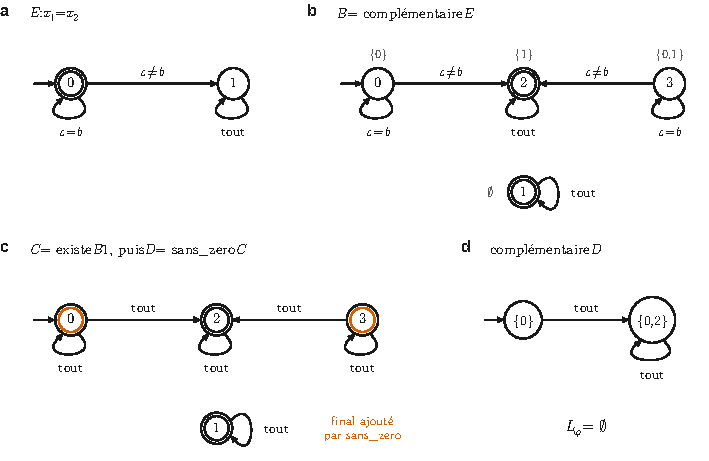
\includegraphics{figures/q27-deroule-automates.pdf}
\caption*{Figure 4 --- Déroulé sur φ(x₂) : (a) E, (b) son complémentaire B, (c)
projection C puis sans\_zero D (finaux ajoutés en vermillon), (d)
complémentaire de D, sans état final accessible}
\end{figure}

C'est cohérent avec la sémantique : \(\varphi(x_2)\) dit que tout entier est égal à \(x_2\), ce qui est toujours faux.

\begin{methode}

Dans un déroulé à la main, ne construisez que la partie accessible des déterminisés, en le disant. Terminez toujours par une vérification sémantique du langage obtenu.

\end{methode}

\hypertarget{question-28}{%
\subsection{Question 28}\label{question-28}}

\begin{indication}{1}

Transcrivez Q26 par un filtrage sur le constructeur.

\end{indication}

\begin{indication}{2}

Le filtrage doit être exhaustif ; l'ordre \texttt{sans\_zero\ (\allowbreak{}automate\_existe\ …)\allowbreak{}} compte.

\end{indication}

\hypertarget{solution-27}{%
\subsubsection{Solution}\label{solution-27}}

\begin{lstlisting}[language=Caml]
let rec automate_formule phi n =
  match phi with
  | Egale (V i, V j) -> automate_egalite n i j
  | Egale (V i, Plus (j, k)) -> automate_somme n j k i     (* x_j + x_k = x_i *)
  | Egale (Plus (j, k), V i) -> automate_somme n j k i     (* cas symetrique *)
  | Egale (Plus _, Plus _) -> failwith "formule non sous forme simple"
  | Non psi -> complementaire (automate_formule psi n)
  | Et (psi1, psi2) ->
      intersection (automate_formule psi1 n) (automate_formule psi2 n)
  | Existe (i, psi) ->
      sans_zero (automate_existe (automate_formule psi n) i)
\end{lstlisting}

Chaque appel récursif porte sur une sous-formule stricte, donc la fonction termine.

\begin{piege}

Appliquer \texttt{sans\_zero} avant la projection ajouterait des zéros sur \textbf{toutes} les lignes, ligne \(i\) comprise : le témoin resterait limité à \(\lvert m\rvert\) bits. Vérifiez aussi l'ordre des arguments de \texttt{automate\_somme}, qui reconnaît \(v_i+v_j=v_k\) pour l'appel \texttt{automate\_somme\ n\ i\ j\ k}.

\end{piege}

\hypertarget{question-29}{%
\subsection{Question 29}\label{question-29}}

\begin{indication}{1}

Procédez par induction structurelle, avec un cas par constructeur.

\end{indication}

\begin{indication}{2}

Établissez d'abord un lemme : ajouter des lettres nulles à droite ne change aucune valeur \(v_j\).

\end{indication}

\begin{indication}{3}

Pour \(\exists\), prouvez une double inclusion entre \(L_{\exists x_i.\psi}\) et l'ensemble des \(m\) dont un prolongement \(m{\mathbf{0}}^p\) est dans \((L_\psi)_{\exists i}\). Choisissez \(p\) assez grand pour écrire le témoin.

\end{indication}

\hypertarget{solution-28}{%
\subsubsection{Solution}\label{solution-28}}

On note \(a_m\) l'assignation \(x_j\mapsto v_j(m)\).

\textbf{Lemme 1.} On a \(v_j(m{\mathbf{0}}^p)=v_j(m)\), donc \(m\in L_\varphi\) si et seulement si \(m{\mathbf{0}}^p\in L_\varphi\).

\textbf{Lemme 2.} Pour \(\varphi=\exists x_i.\psi\), on a
\equationajustee{L_\varphi=\{m:\exists p,\ m{\mathbf{0}}^p\in(L_\psi)_{\exists i}\}.}

\begin{itemize}
\tightlist
\item
  (\(\subseteq\)) Soit \(N\) un témoin. On choisit \(p\) avec \(N<2^{\lvert m\rvert+p}\).

  \begin{itemize}
  \tightlist
  \item
    Soit \(w\) égal à \(m{\mathbf{0}}^p\) hors de la ligne \(i\), avec la ligne \(i\) égale à l'écriture binaire de \(N\).
  \item
    Par le lemme 1, \(a_w\) coïncide avec \(a_m[x_i\mapsto N]\) sur les variables libres de \(\psi\), donc \(w\in L_\psi\).
  \end{itemize}
\item
  (\(\supseteq\)) Si un tel \(w\in L_\psi\) existe, alors \(N=v_i(w)\) est un témoin.
\end{itemize}

\textbf{Lemme 3.} \texttt{sans\_zero} \(\mathcal{A}\) reconnaît \(\{m:\exists p,\ m{\mathbf{0}}^p\in\mathcal{L}(\mathcal{A})\}\). Cela découle de Q23 et de
\equationajustee{\widehat{\delta}(q_0,m{\mathbf{0}}^p)=\bigcup_{q\in\widehat{\delta}(q_0,m)}\widehat{\delta}(q,{\mathbf{0}}^p).}

\textbf{Théorème.} L'automate \texttt{automate\_formule\ phi\ n} reconnaît \(L_\varphi\). Preuve par induction structurelle :

\begin{itemize}
\tightlist
\item
  \textbf{Atomes} : par hypothèse sur les automates fournis. En effet, \([\![x_i=x_j]\!]_{a_m}\) est vraie si et seulement si \(v_i(m)=v_j(m)\), et de même pour la somme.
\item
  \textbf{\(\neg\psi\)} : \(L_{\neg\psi}=\Sigma_n^*\setminus L_\psi\), et Q13 conclut.
\item
  \textbf{\(\psi_1\wedge\psi_2\)} : \(a_m\) donne la même valeur à \(x_j\) dans les deux sous-formules, même si leurs variables libres diffèrent. Donc \(L_\varphi=L_{\psi_1}\cap L_{\psi_2}\), et Q14 conclut.
\item
  \textbf{\(\exists x_i.\psi\)} : l'hypothèse d'induction et Q25 donnent un automate pour \((L_\psi)_{\exists i}\), puis les lemmes 3 et 2 concluent.
\end{itemize}

\begin{methode}

Une preuve de correction par induction structurelle traite tous les constructeurs et énonce l'hypothèse d'induction. Le cas délicat, ici le quantificateur, demande une vraie double inclusion : c'est là qu'intervient \texttt{sans\_zero}.

\end{methode}

\hypertarget{question-30}{%
\subsection{Question 30}\label{question-30}}

\begin{indication}{1}

Sans variable libre, que peut valoir \(L_\varphi\) ?

\end{indication}

\begin{indication}{2}

Un seul mot suffit alors à décider. Lequel est le plus simple à tester, compte tenu de la convention sur l'état initial ?

\end{indication}

\hypertarget{solution-29}{%
\subsubsection{Solution}\label{solution-29}}

Si \(\varphi\) est close, \([\![\varphi]\!]_{a_m}\) ne dépend pas de \(m\). Donc \(L_\varphi=\Sigma_n^*\) si \(\varphi\) est vraie, et \(L_\varphi=\emptyset\) sinon.

Il suffit de tester \(\varepsilon\), qui est accepté si et seulement si l'état initial, l'état \(0\), est final.

\begin{lstlisting}[language=Caml]
let est_vraie phi n =
  (automate_formule phi n).finaux.(0)
\end{lstlisting}

\textbf{\(\varphi\) est vraie si et seulement si l'état 0 de l'automate de Q28 est final.} La lecture du bit est immédiate ; tout le coût est dans la construction de l'automate, qui déterminise à chaque négation et peut donc être gigantesque.

\begin{piege}

Cette lecture n'est juste que si \texttt{determinise} respecte la convention « état initial = état 0 » (Q12). Il ne faut pas non plus présenter la décision comme rapide : avec des négations imbriquées, le nombre d'états croît comme une tour d'exponentielles.

\end{piege}

\hypertarget{bilan}{%
\section{Bilan}\label{bilan}}

\textbf{Ce que le rapport 2026 met en avant.} Le reproche dominant est le refus du formalisme : en Q10, Q14 et Q20, les réponses en langage courant sont jugées approximatives ou incomplètes. Viennent ensuite les preuves à deux sens (Q5, Q16), les complexités affirmées sans lien avec le code (Q2), les automates remplis à moitié (Q15) et le lemme de l'étoile mal énoncé (Q17). Le rapport insiste aussi sur la présentation : copies lisibles, noms significatifs, fonctions auxiliaires, commentaires.

\textbf{Méthodes à retenir.}

\begin{itemize}
\tightlist
\item
  \textbf{Codage binaire, poids faible en tête} : il permet de lire un nombre au fil d'un mot. L'égalité de deux lignes d'un même mot équivaut à l'égalité des valeurs, et ajouter des zéros à droite ne change rien.
\item
  \textbf{Prouver un automate} : décrire ses mots sous forme régulière (Q5), ou donner un sens numérique à chaque état sur les préfixes et prouver une équivalence à chaque pas (Q7, Q16).
\item
  \textbf{Constructions sur les automates} : déterminisation par sous-ensembles, complémentaire (seulement sur un automate déterministe complet), produit pour l'intersection, projection d'une composante, saturation par point fixe. Ce sont des briques réutilisables.
\item
  \textbf{Conventions d'implémentation} : un codage des états doit respecter les conventions du type, comme l'état initial numéroté 0 en Q12. Les erreurs silencieuses de ce genre se paient plus loin.
\item
  \textbf{Non-reconnaissabilité} : lemme de l'étoile, énoncé avec ses trois conditions, appliqué à un mot dont la zone pompable est neutre (Q17).
\item
  \textbf{Logique} : définir des constantes sans constantes (Q19), traiter le cas atomique d'une induction sur les formules (Q20), lire correctement des règles nouvelles comme \({\mathrm{sub}}_=\) et \(\mathrm{cut}\) (Q22).
\end{itemize}

\textbf{Prérequis à revoir.} Le cours sur les automates (déterminisation, clôtures, lemme de l'étoile), les preuves par induction structurelle, la déduction naturelle avec les règles \(\vee e\), \(\neg e\) et \(\bot\), et le filtrage OCaml sur listes et types somme.

\textbf{Questions transposables.} L'exponentiation rapide et sa complexité, la déterminisation codée par des entiers, le complémentaire, le produit d'automates et l'automate de l'addition binaire se retrouvent dans de nombreux sujets. La non-reconnaissabilité d'une relation arithmétique est un classique, de même que la traduction formule → automate, qui est la méthode de Büchi pour décider l'arithmétique de Presburger.

\end{document}
